\begin{figure}[H]
    \centering
    \begin{subfigure}[t]{0.45\textwidth}
        \centering
        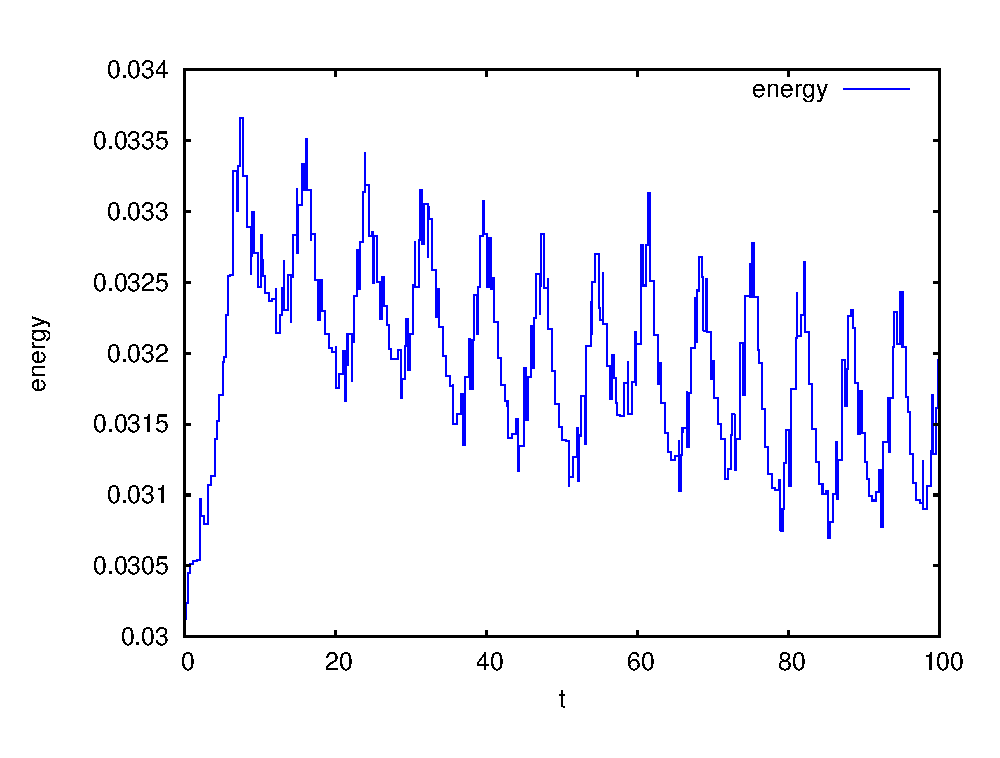
\includegraphics[width=\linewidth]{pic/rol__wrench__kinetic_energy}
        \caption{Кинетическая энергия}
        \label{fig:rol__wrench__kinetic_energy}
    \end{subfigure}
    \begin{subfigure}[t]{0.45\textwidth}
        \centering
        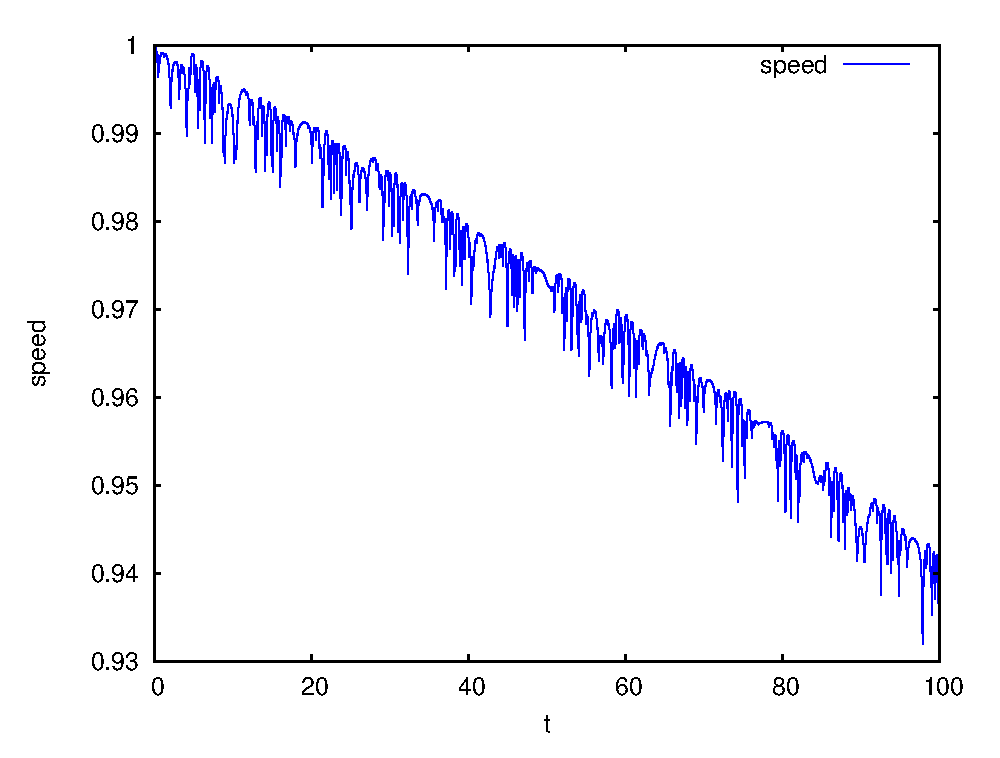
\includegraphics[width=\linewidth]{pic/rol__wrench__speed_of_center_of_mass}
        \caption{Скорость центра масс $\left(\nu_1^2 + \nu_2^2\right)(t)$}
        \label{fig:rol__wrench__speed_of_center_of_mass}
    \end{subfigure}
    \vspace{12pt}
    
    \begin{subfigure}[t]{0.45\textwidth}
        \centering
        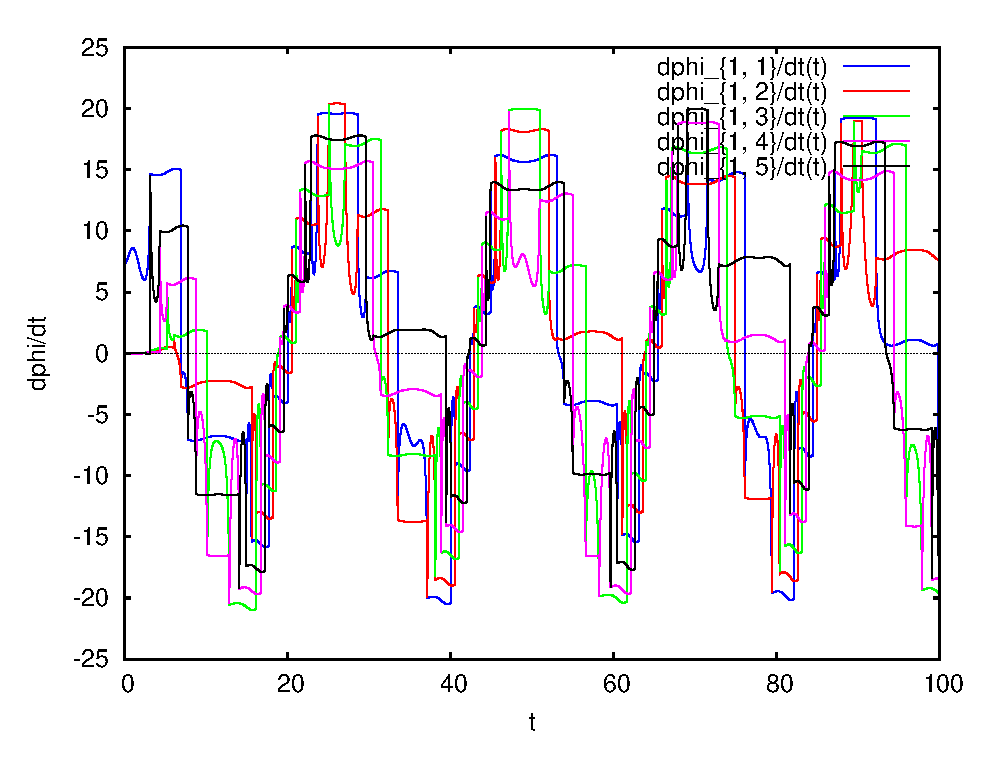
\includegraphics[width=\linewidth]{pic/rol__wrench__velocities_of_rollers_of_wheel_1}
        \caption{Скорости роликов $\dot{\phi}_{ij}(t)$ на первом колесе}
        \label{fig:rol__wrench__velocities_of_rollers_of_wheel_1}    
    \end{subfigure}
    \hfill
    \begin{subfigure}[t]{0.45\textwidth}
        \centering
        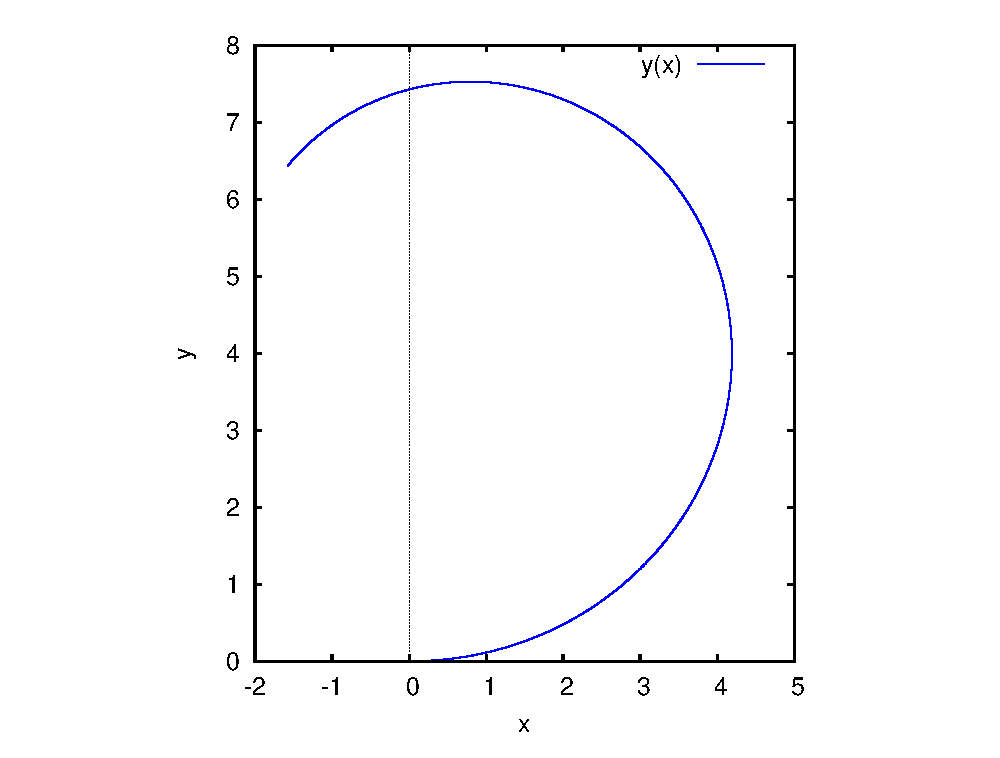
\includegraphics[width=\linewidth]{pic/rol__wrench__trajectory} \\
        \caption{Траектория центра масс на плоскости $OXY$}
        \label{fig:rol__wrench__trajectory}
    \end{subfigure}
    
    \caption{Экипаж c роликами. Движение с закруткой ($\nu_1(0) = 1, \nu_2(0) = 0, \nu_3(0) = 1$).}
    \label{fig:wrench}
    
\end{figure}
